\documentclass[final]{fhnwreport}       %[mode] = draft or final
                                        %{class} = fhnwreport, article, 
                                        %          report, book, beamer, standalone
%%---Main Packages-----------------------------------------------------------------------
\usepackage[english, ngerman]{babel}	%Mul­tilin­gual sup­port for LaTeX
\usepackage[T1]{fontenc}				%Stan­dard pack­age for se­lect­ing font en­cod­ings
\usepackage[utf8]{inputenc}				%Ac­cept dif­fer­ent in­put en­cod­ings
\usepackage{lmodern}                    %The newer Font-Set
\usepackage{textcomp}					%LaTeX sup­port for the Text Com­pan­ion fonts
\usepackage{graphicx} 					%En­hanced sup­port for graph­ics
\usepackage{float}						%Im­proved in­ter­face for float­ing ob­jects
\usepackage{ifdraft}                    %Let you check if the doc is in draft mode

%%---Useful Packages---------------------------------------------------------------------
\usepackage[pdftex,dvipsnames]{xcolor}  %Driver-in­de­pen­dent color ex­ten­sions for LaTeX
\usepackage{csquotes}                   %Simpler quoting with \enquote{}
\usepackage{siunitx} 					%A com­pre­hen­sive (SI) units pack­age
\usepackage{listings}					%Type­set source code list­ings us­ing LaTeX
\usepackage[bottom]{footmisc}			%A range of foot­note op­tions
\usepackage{footnote}					%Im­prove on LaTeX's foot­note han­dling
\usepackage{verbatim}					%Reim­ple­men­ta­tion of and ex­ten­sions to LaTeX ver­ba­tim
\usepackage[textsize=footnotesize]{todonotes} %Mark­ing things to do in a LaTeX doc­u­ment

%%---Tikz Packages-----------------------------------------------------------------------
\usepackage{standalone}
\usepackage{tikz}
\usepackage{circuitikz}
\usetikzlibrary{arrows}
\usetikzlibrary{calc}
\usetikzlibrary{intersections}

%%---Math Packages-----------------------------------------------------------------------
\usepackage{amsmath}					%AMS math­e­mat­i­cal fa­cil­i­ties for LaTeX
%\usepackage{amssymb}					%Type­set­ting symbols (AMS style)
%\usepackage{array}						%Ex­tend­ing the ar­ray and tab­u­lar en­vi­ron­ments
%\usepackage{amsthm}					%Type­set­ting the­o­rems (AMS style)

%%---Table Packages----------------------------------------------------------------------
\usepackage{tabularx}					%Tab­u­lars with ad­justable-width columns
%\usepackage{longtable}
\usepackage{multirow}					%Create tab­u­lar cells span­ning mul­ti­ple rows
\usepackage{multicol}					%In­ter­mix sin­gle and mul­ti­ple columns

%%---PDF / Figure Packages---------------------------------------------------------------
\usepackage{pdfpages}					%In­clude PDF doc­u­ments in LaTeX
\usepackage{pdflscape}					%Make land­scape pages dis­play as land­scape
\usepackage{subfig}					    %Fig­ures di­vided into sub­fig­ures

%%---Other Packages----------------------------------------------------------------------
%\usepackage{xargs}                     %De­fine com­mands with many op­tional ar­gu­ments

%%---Bibliography------------------------------------------------------------------------
\usepackage[style=ieee,urldate=comp,backend=biber]{biblatex}
\addbibresource{literature/bibliography.bib}

%%---Main Settings-----------------------------------------------------------------------
\graphicspath{{./graphics/}}			%Defines the graphicspath
%\geometry{twoside=false}				    %twoside=false disables the "bookstyle"
\setlength{\marginparwidth}{2cm}
\overfullrule=5em						%Creates a black rule if text goes over the margins => debugging


%%---User Definitions--------------------------------------------------------------------
%%Tabel-Definitions: (requires \usepackage{tabularx})
\newcolumntype{L}[1]{>{\raggedright\arraybackslash}p{#1}}    %column-width and alignment
\newcolumntype{C}[1]{>{\centering\arraybackslash}p{#1}}
\newcolumntype{R}[1]{>{\raggedleft\arraybackslash}p{#1}}

%%---Optional Package Settings-----------------------------------------------------------
%Listings-Settings: (requires \usepackage{listings}) => Example with Matlab Code
\lstset{language=Matlab,%
    basicstyle=\footnotesize\ttfamily,
    breaklines=false,%
    morekeywords={switch, case, otherwise},
    keywordstyle=\color{Blue},%
    tabsize=2,
    %morekeywords=[2]{1}, keywordstyle=[2]{\color{black}},
    identifierstyle=\color{Black},%
    stringstyle=\color{Purple},
    commentstyle=\color{Green},%
    showstringspaces=false,%without this there will be a symbol in the places where there is a space
    numbers=left,%
    numberstyle={\tiny \color{black}},% size of the numbers
    numbersep=9pt, % this defines how far the numbers are from the text
    %emph=[1]{word1, word2,...},emphstyle=[1]\color{red}
}										                %loads all packages, definitions and settings												
\title{Pflichtenheft}          %Project Title
\author{Projekt 5}          %Document Type => Technical Report, ...
\date{Windisch, {\today}}             %Place and Date

\begin{document}
%%---TITLEPAGE---------------------------------------------------------------------------
\selectlanguage{ngerman}                %ngerman or english
\maketitle

\vspace*{-1cm}						    %compensates the space after the date line.
\vfill
\begin{figure}[H]
\centering

\includegraphics[width=\linewidth]{titelbild_p5.jpg}
\end{figure}
\vfill

{
\renewcommand\arraystretch{2}
\begin{center}
\begin{tabular}{>{\bf}p{4cm} l}
Hochschule                 &    Hochschule für Technik - FHNW\\
Studiengang                &    Elektro- und Informationstechnik\\
Autor   		           & 	Adrian Annaheim und Simon Zoller\\
Betreuer                   &    Pascal Schleuniger\\
Auftraggeber               &    Ferrum AG\\
Version                    &    0.0 %Normally not used!
\end{tabular}
\end{center}
}

\clearpage
			
%%---ABSTRACT----------------------------------------------------------------------------
\selectlanguage{ngerman}				%ngerman or english
\thispagestyle{empty}
%\begin{abstract}
Das Abstract ist eine Art Zusammenfassung des ganzen Dokuments. Es gibt einen Einblick in die Aufgabenstellung, wie diese umgesetzt wurde und welches Ergebnis erreicht wurde. Aus diesem Grund wird das Abstract immer ganz am Schluss der Arbeit verfasst. Es besteht aus einem zusammengehörenden Absatz und umfasst ungefähr 10 bis 20 Zeilen.
Formeln, Referenzen oder andere Unterbrechungen haben im Text nichts zu suchen.
Direkt unter dem Abstract folgt eine Liste von drei bis vier Stichworten/Keywords. Diese werden in alphabetischer Reihenfolge aufgelistet und beschreiben das Themengebiet der Arbeit.

\vspace{2ex}
\textbf{Keywords: Anleitung, LaTeX, Thesis, Vorlage}
\end{abstract}	


\vfill

\begin{center}
\color{green!50!black!100}\bf
Bitte schicken Sie jeglichen Feedback auch an \texttt{hanspeter.schmid@fhnw.ch}\\
Er wird dieses Template langfristig unterhalten.
\end{center}

\vfill
\null

%%---TABLE OF CONTENTS-------------------------------------------------------------------
\pagenumbering{Roman}		
\selectlanguage{ngerman}				%ngerman or english
\tableofcontents
\clearpage

%%---TEXT--------------------------------------------------------------------------------
\pagenumbering{arabic}
\section{Projektziele}

Das übergeordnete Ziel dieses Projektes ist ein Versuchsaufbau zur berührungslosen Energie- und Datenübertragung zu realisieren. Dafür wurden mehrere Sollziele definiert.
\section*{Sollziele}
\begin{table}[h]
\centering

	\begin{tabular}{c|c|l}
	\textbf{Punkt} & \multicolumn{2}{c}{\textbf{Sollziele}} \\
	\hline
	S1 & \multicolumn{2}{l}{Analyse und Dimensionierung für einen induktiven Drehübertrager 300W/48V} \\
	\hline
	S2 & \multicolumn{2}{l}{Laboraufbau und Simulation induktive Drehübertragung} \\
	\hline
	S3 & \multicolumn{2}{l}{mindestens 300W/48V sollen mit dem Laboraufbau induktiv übertragen werden} \\
	\hline
	S4 & \multicolumn{2}{l}{Analyse VARAN-Bus} \\
	\hline
	S5 & \multicolumn{2}{l}{\begin{tabular}[c]{@{}l@{}}Es soll ein Konzept erarbeitet werden, um Daten des VARAN-Buses \\ bidirektional und optisch zu übertragen\end{tabular}} \\
	\hline
	S6 & \multicolumn{2}{l}{\begin{tabular}[c]{@{}l@{}}Testaufbau zur optischen Datenübertragung, welcher die Spezifikationen des \\ VARAN-Buses erfüllt\end{tabular}} \\
%	S6 & \multicolumn{2}{l}{Testaufbau zur optischen Datenübertragung, welcher die Spezifikationen des VARAN-Buses erfüllt} \\
	\end{tabular}
\caption{}
\label{tab:sollziele}
\end{table}

\section*{Wunschziele}
\begin{table}[h]
	\centering
	\begin{tabular}{c|c|l}
	\textbf{Punkt} & \multicolumn{2}{c}{\textbf{Sollziele}} \\
	\hline
	W1 & \multicolumn{2}{l}{Optische Datenübertragung über maximal zwei Kanäle} \\	
	\end{tabular}
\caption{}
\label{tab:wunschziele}
\end{table}
\section{Zeitplan}

\begin{figure}[H]
\centering
\includegraphics[angle=90,width=\textwidth]{zeitplan.png}
\end{figure}
\section{Projektvereinbarung}

Betreuender Dozent \bigskip \\
Prof. Dr. Pascal Schleuniger \bigskip \\
Ort, Datum\hspace{3cm} Unterschrift \bigskip \\
\rule{4cm}{0.4pt} \hspace{0.9cm} \rule{4cm}{0.4pt}\bigskip \\

Student \bigskip \\
Adrian Annaheim \bigskip \\
Ort, Datum\hspace{3cm} Unterschrift \bigskip \\
\rule{4cm}{0.4pt} \hspace{0.9cm} \rule{4cm}{0.4pt}\bigskip \\

Student \bigskip \\
Simon Zoller \bigskip \\
Ort, Datum\hspace{3cm} Unterschrift \bigskip \\
\rule{4cm}{0.4pt} \hspace{0.9cm} \rule{4cm}{0.4pt}\bigskip \\



%\section{Tikz-Grafiken}
Tikz ist ebenfalls sehr mächtig und auf den ersten Blick auch sehr kompliziert. Schon alleine die Dokumentation des Grundpackages erstreckt sich über 1000 Seiten. Tikz lohnt sich vor allem, wenn die erstellte Grafik (oder nur Teile davon) wiederverwendet werden können.
Es folgen drei Beispiele für Tikz-Grafiken.

Man beachte, dass diese in einem eigenen \enquote{\LaTeX-Projekt} erstellt wurden. Dieses hat die \verb|\documentclass{standalone}| und kann deswegen eigenständig kompiliert werden. Dabei werden automatisch Unterstüzungslinien/Grid eingeblendet (wurde programmiert), welche die Gestaltung der Grafik extrem erleichtern. Schaut euch doch die Tikz-Dateien an und kompiliert sie separat, es lohnt sich!

Mittels Befehl \verb|\includestandalone{}| werden dann diese in jedes andere Projekte eingebunden, und zwar nicht als PDF sondern direkt erstellt beim Kompilieren.

Somit können wir nun einfache elektrische Schaltungen wie in Figur~\ref{subfig:einfach} oder auch komplizierte Blockschaltbilder wie in Figur~\ref{subfig:kompliziert} programmieren.

\begin{figure}[b]
\centering
\subfloat[Einfach]{\includestandalone{tikz/beispiel1}\label{subfig:einfach}}

\subfloat[Kompliziertes Blockschaltbild]{\includestandalone{tikz/beispiel2}\label{subfig:kompliziert}}

\caption{Zwei tikz-Beispiele: \protect\subref{subfig:einfach} einfach, \protect\subref{subfig:kompliziert} kompliziert.}
\label{fig:tikz}
\end{figure}

Im Dokumenteordner \mbox{\emph{/tikz/}} findet ihr noch zwei weitere Beispiele. Eines zeigt ein \textbf{animiertes Tikz} und das andere interagiert mit \textbf{gnuplot}, um Plots zur Laufzeit zu erstellen. Um gnuplot nutzen zu können sind ein paar zusätzliche Installationen notwendig. Weiter muss der Kompilierbefehl für \texttt{pdflatex} mit \texttt{--shell-escape} erweitert werden. Das Internet bietet gute Unterstützung bei der Integration von gnuplot.
Viele weitere coole Beispiele findet ihr auf \mbox{http://www.texample.net/tikz/examples/}.


%\section{Bibliographien}
Dieses Template arbeitet mit bibLaTeX und biber; einige Informationen dazu findet man in \cite{biblatex_biber}. Die Anwendung \texttt{biber.exe} ist standardmässig installiert, muss jedoch anstelle von \texttt{bibtex.exe} aufgerufen werden. \textbf{Dazu muss im verwendeten Editor der Bib(la)tex Befehl durch biber ersetzt werden.} 

\subsection{Literaturdatenbank}
Um zu Referenzieren braucht man nun nur die Datei \verb|literature/bibliography.bib| auszufüllen (BibLaTeX-Mode), zum Beispiel mit Hilfe des Quellenverwaltungsprogramm JabRef \cite{jabref}. Danach muss das Dokument mehrfach zu kompilieren: einmal mit pdfLaTeX, damit die Literaturverweise erkannt und festgehalten werden, dann einmal mit biber, welches die Daten aus \verb|literature/bibliography.bib| herausliest und in das richtige Format bringt, und dann zweimal mit pdfLaTeX, damit das Literaturverzeichnis korrekt wird und alle Nummern im Text stimmen.

\subsection{Referenzieren}
Man kann nun mit verschiedenen Versionen des Befehles \verb|\cite| nun einzelne Publikationen \cite{Mason1953}, mehrere miteinander \cite{Mason1953,Mason1956}, oder Abschnitte aus einer Publikation \cite[Sec.~4]{Schmid2018} zitieren.
Für die genaue Positionierung der Referenzen bitte den Leitfaden verwenden.

\subsection{Literaturverzeichnis}
Der Befehl \verb|\printbibliography| erstellt ein Literaturverzeichnis.
Wie auf Seite~\pageref{sec:lit} zu sehen ist, passt sich das Literaturverzeichnis so automatisch der gewählten Sprache an.

\subsection{Was bedeutet eigentlich zitieren und referenzieren?}

\paragraph{Woher habe ich meine Information?}
Meine Ansichten darüber, wie Wissenschaft funktioniert, decken sich weitgehend mit \cite{Schmid2003}.

\paragraph{Woher genau?}
Die genaue Zusammenstellung der drei Kriterien für empirische Wissenschaftlichkeit ist zu finden in \cite[S.~80]{Schmid2003}

\paragraph{Was steht denn dort?}
Praphrasieren: In \cite{Schmid2003} beschreibt Schmid, dass es für empirische Wissenschaften nicht nur wesentlich ist, sich auf die Wirklichkeit zu beziehen und sich darüber Gedanken zu machen, sonder auch diese Gedanken mit anderen Wissenschaftlern zu teilen und zu besprechen.

\paragraph{Was steht denn dort \emph{genau}?}
In \cite{Schmid2003} steht:
\begin{quote}
\selectlanguage{english}				%ngerman or english
All that is empirical science has three things in
common: a practical injunction (if you want to know
this, you have to do this); an apprehension, illumination, or experience (if you do this, you see this), and communal checking (did others who did this also see the same?).
\end{quote}
Das habe ich oben gemeint mit \enquote{[ \ldots ] dass es für empirische Wissenschaften nicht nur wesentlich ist, sich auf die Wirklichkeit zu beziehen und sich darüber Gedanken zu machen, sonder auch diese Gedanken mit anderen Wissenschaftlern zu teilen und zu besprechen.}

\paragraph{Und wenn jemand einen Fehler gemacht hat?}
Tellegen publizierte das 1954 schon in seinem Paper \emph{La recherche pour una [sic!] s{\'e}rie compl{\`e}te d’{\'e}l{\'e}ments de circuit ideaux non-lin{\'e}aires} \cite{Tellegen1954}.

%%---BIBLIOGRAPHY------------------------------------------------------------------------
{\sloppypar
\printbibliography[heading=bibintoc]
\label{sec:lit}
\selectlanguage{english}				%ngerman or english
\printbibliography[heading=bibintoc]
}

%%---APPENDIX----------------------------------------------------------------------------
%\begin{appendix} %Anhang

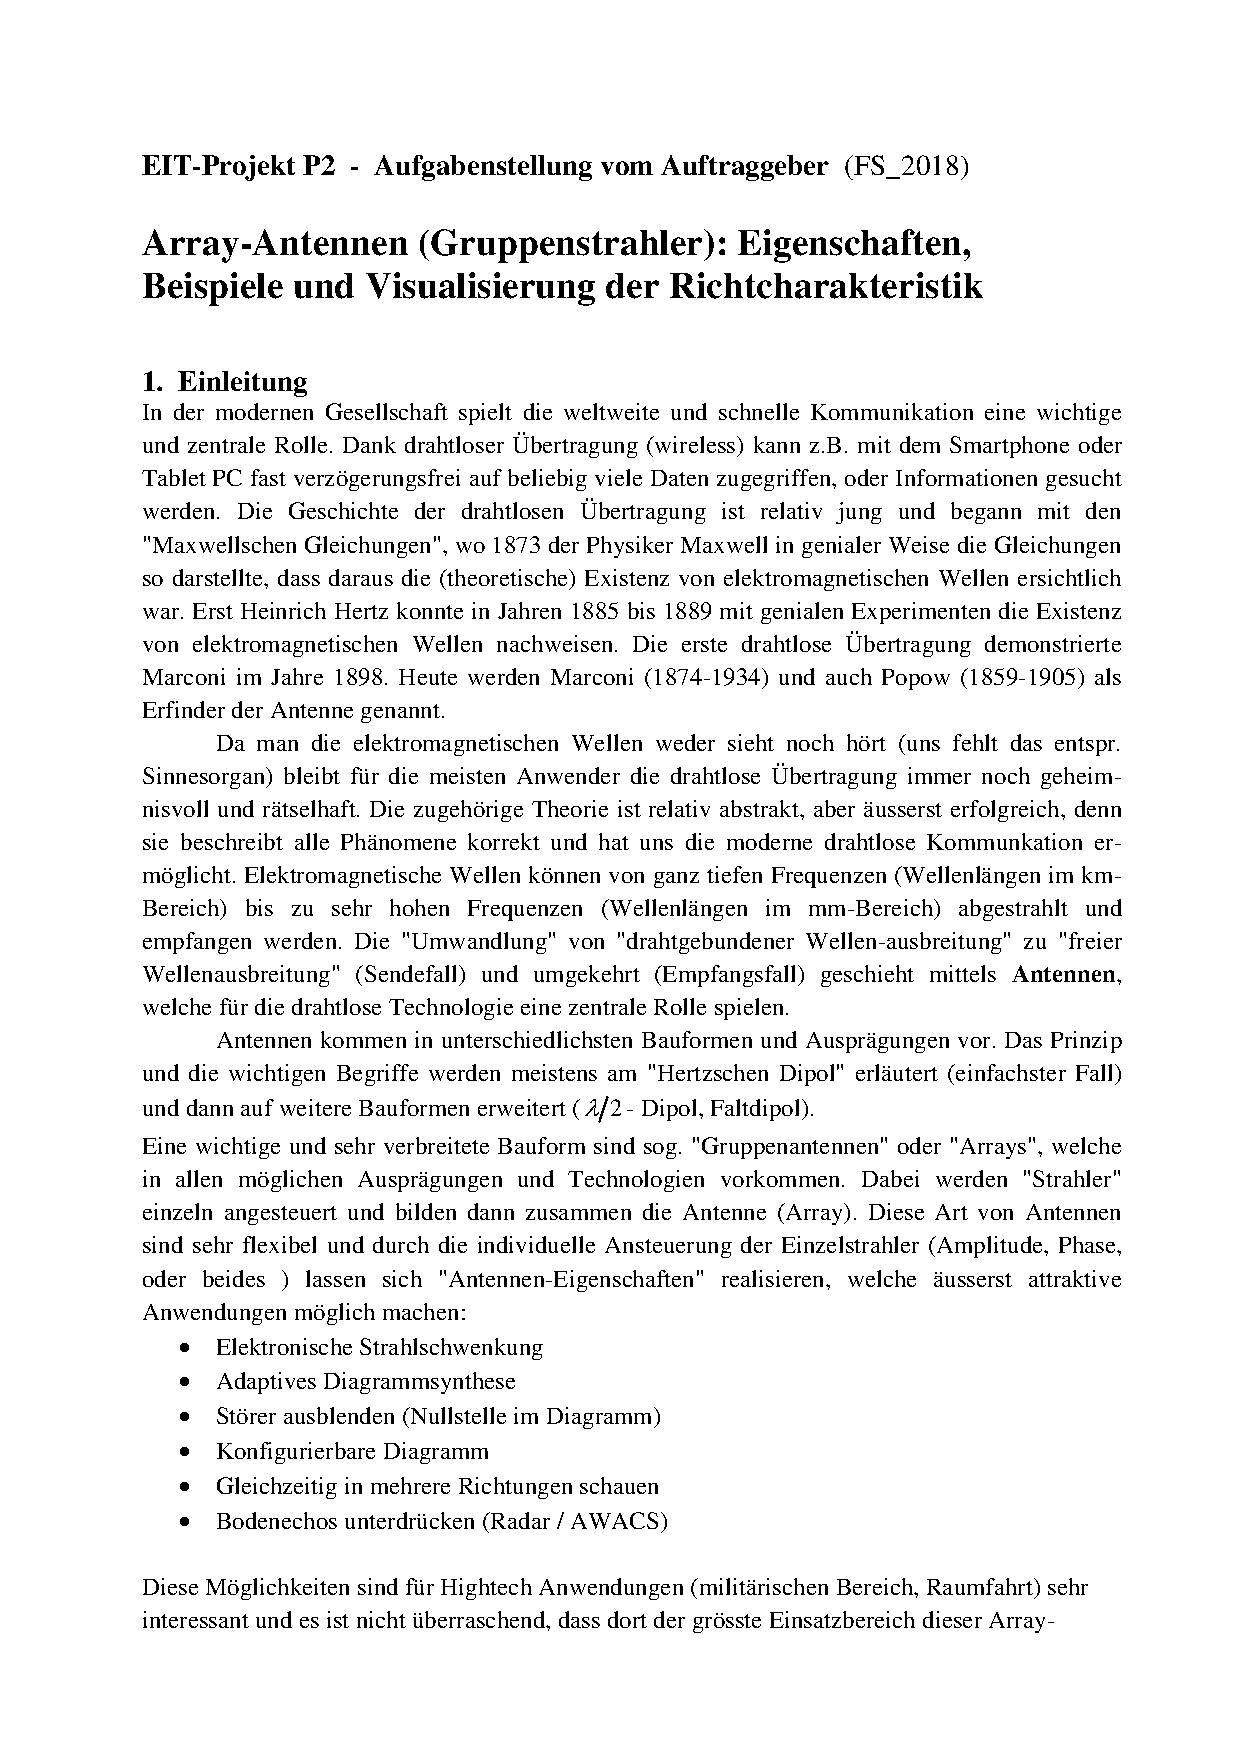
\includepdf[pages={1-2},nup=1x2,landscape=true,scale=0.85,offset=10 -40,pagecommand={\section{Eingefügtes Dokument; zwei Seiten auf einer}\label{app:Aufgabenstellung}\thispagestyle{myheadings}}]{appendix/aufgabenstellung.pdf} \newpage
%%Bei mehrseitigen Dokumenten die folgenden Seiten ohne Überschrift:
%\includepdf[pages={3-6},nup=1x2,landscape=true,scale=0.85,offset=10 -40,pagecommand={\thispagestyle{myheadings}}]{appendix/aufgabenstellung.pdf} \newpage

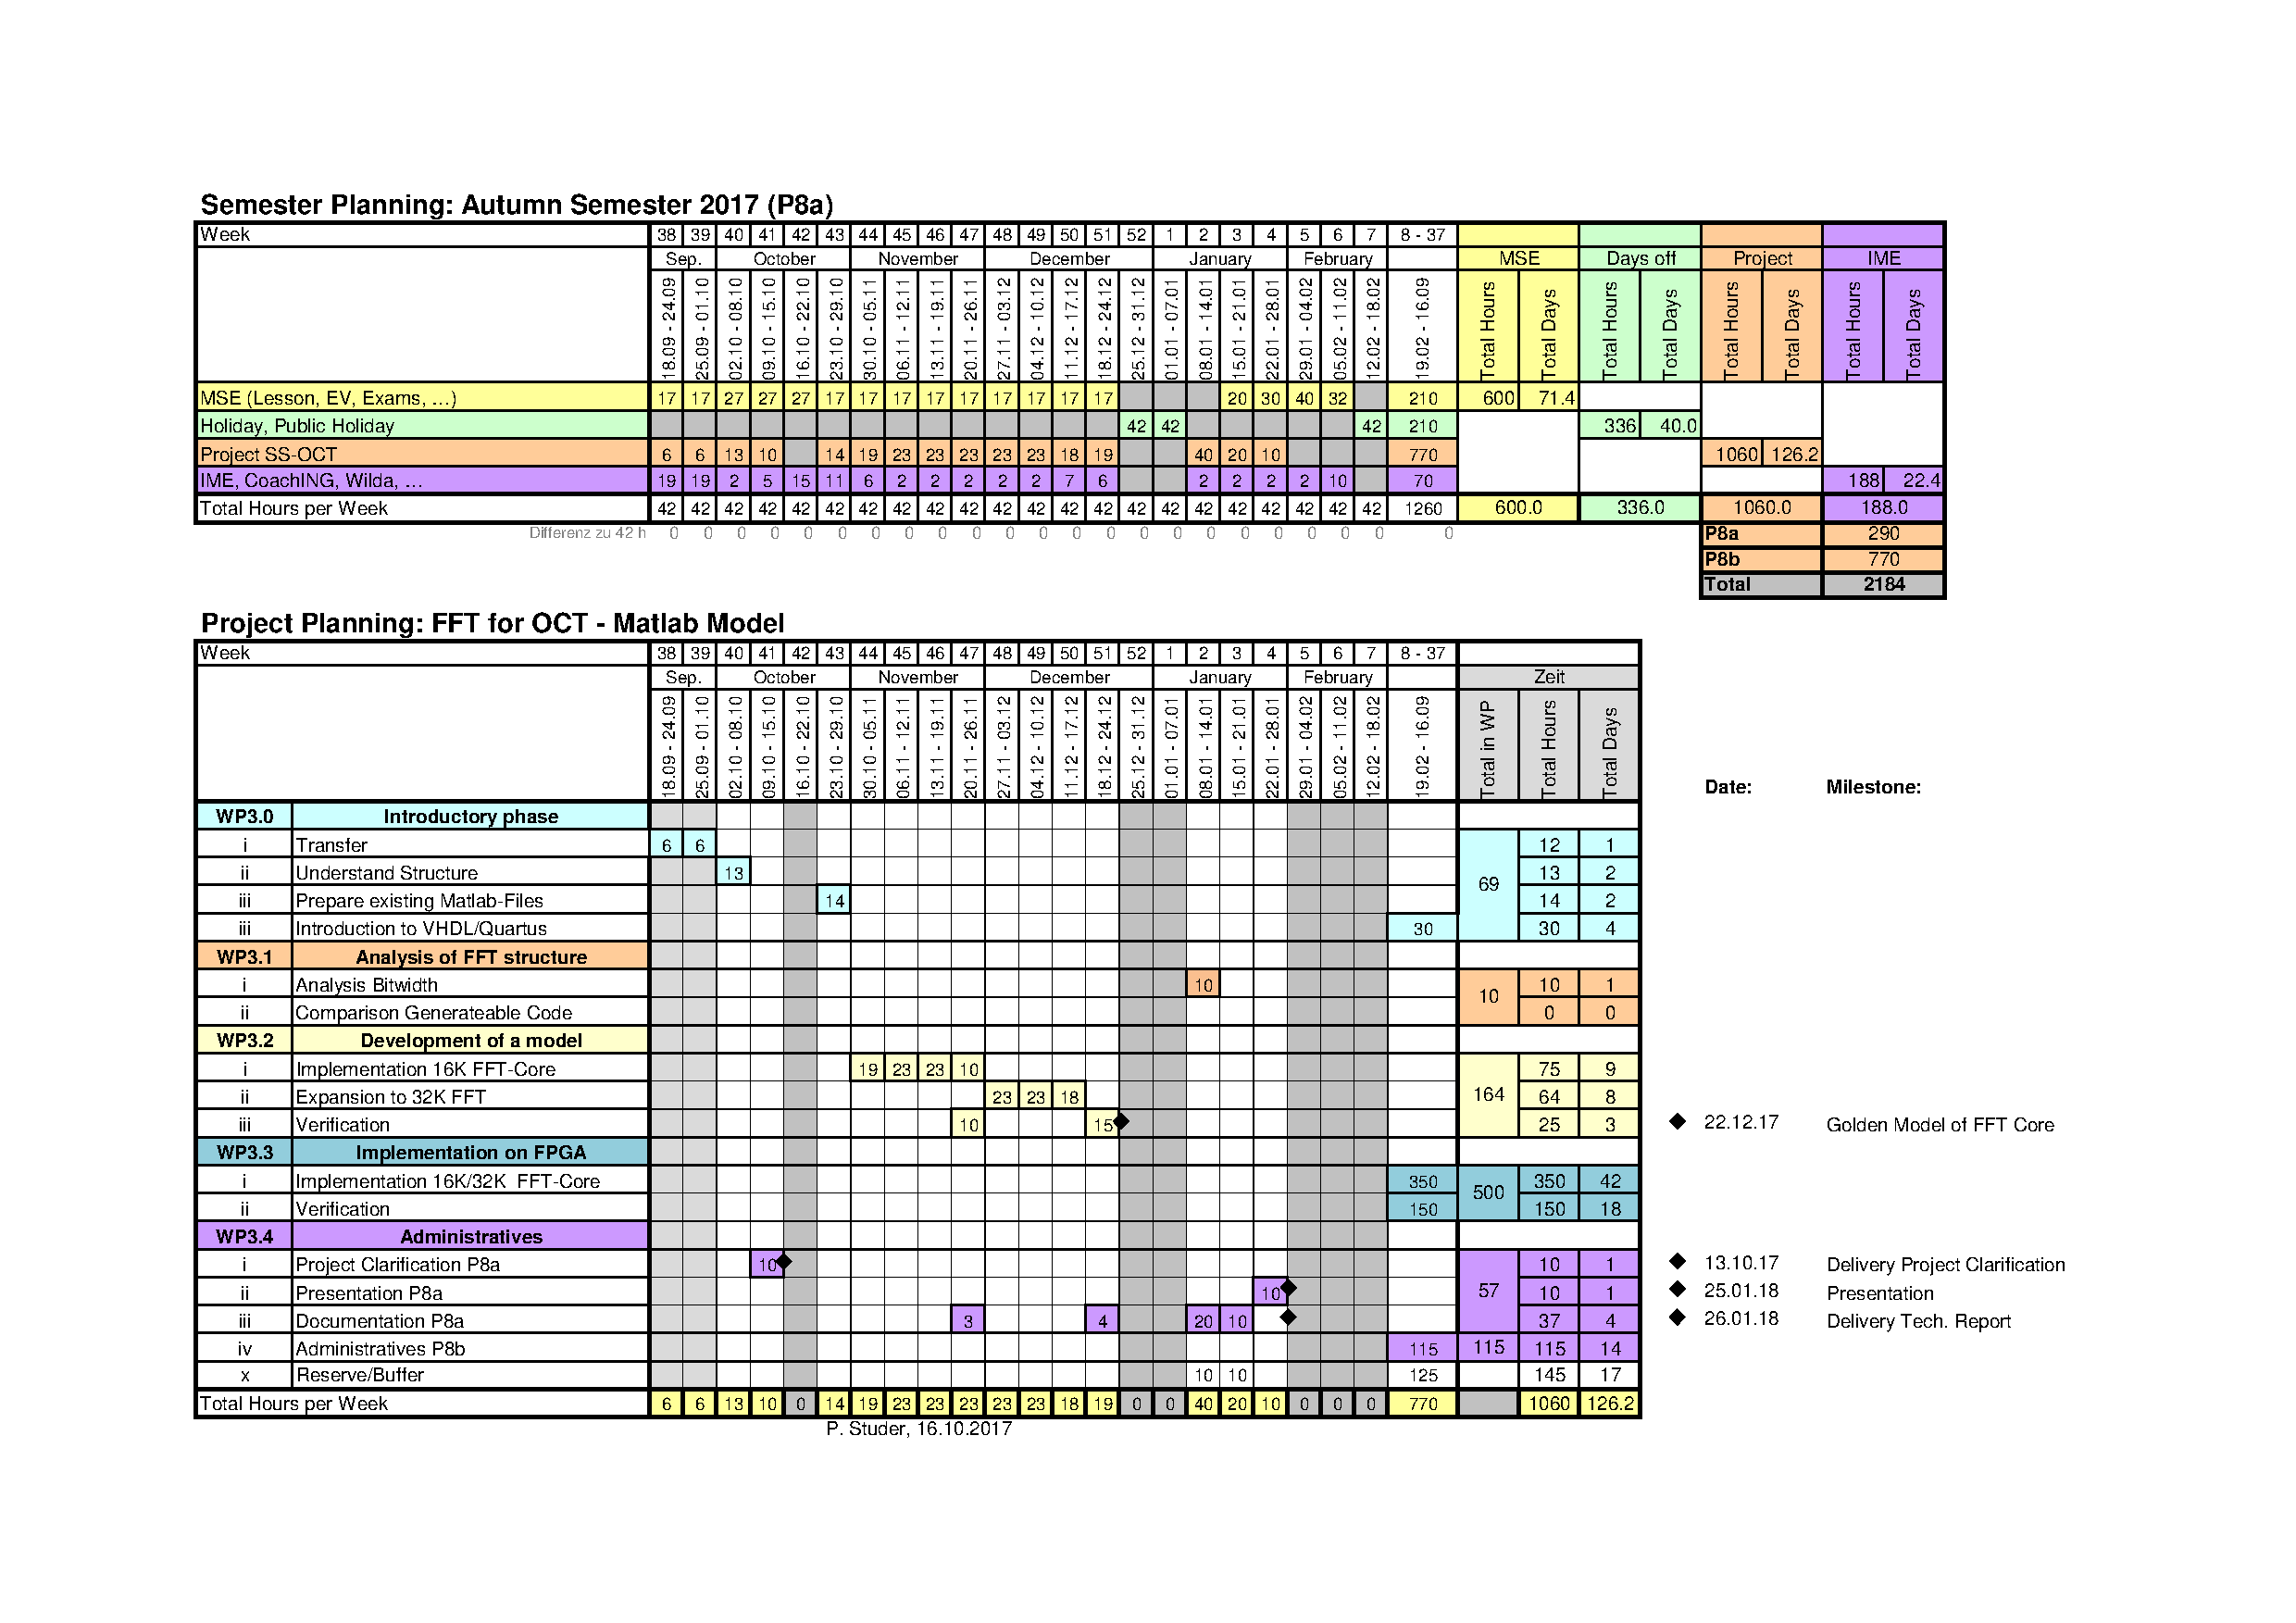
\includepdf[pages={1},nup=1x1,landscape=true,scale=0.85,offset=10 -40,pagecommand={\section{Eingefügte PDF-Tabelle}\label{app:Timetable}\thispagestyle{myheadings}}]{appendix/timeline_example.pdf} \newpage
%%Bei mehrseitigen Dokumenten die folgenden Seiten ohne Überschrift:
%\includepdf[pages={2-5},nup=1x1,landscape=true,scale=0.85,offset=0 -20,pagecommand={\thispagestyle{myheadings}}]{appendix/timeline_example.pdf} \newpage

\section{MATLAB-Code Snippets}
\lstinputlisting{appendix/code/matlab.m}


\end{appendix}


%%---NOTES for DEBUG---------------------------------------------------------------------
\ifdraft{%Do this only if mode=draft
%%requires \usepackage{todonotes})
\newpage
\listoftodos[\section{Todo-Notes}]
\clearpage
}
{%Do this only if mode=final
}
\end{document}
